\section{Introduction}
\label{sec:introduction}

This project is a case study of certain AOCS equipment of a LEO satellite, in particular a BASS Coarse Sun Sensor (CSS) and an AOCS controller.
The simulation will be based on the \textit{SimTG Simulation Modeling Framework}, which is provided by \textit{Airbus Defence and Space} in the \textit{Eclipse} IDE. 

\begin{figure}[h]
    \centering
    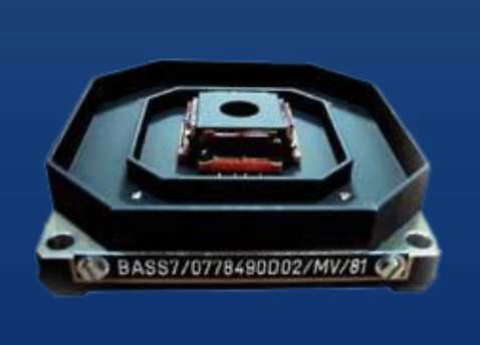
\includegraphics[width=0.5\linewidth]{Graphics/BASS.png}
    \caption{BASS sun sensor from assignment}
    \label{fig:bass}
\end{figure}

To install the SimTG framework, a download link from Airbus Defence and Space is required to get the \texttt{simtg.tgz} installation file.
This installation file must then be extracted on the simulation computer, which needs to run on the \textit{Linux Ubuntu version 16.04.07} operating system. 
For the implementation of this project, the Ubuntu version was installed on a virtual machine using the \textit{Oracle VM Virtual Machine} software. 
Finally, once the SimTG framework has been extracted, it can be run with the \texttt{./simtg.sh} shell script from within the extracted framework directory \texttt{simtg}.
The executables for the simulation are developed in \texttt{C++}, with the test being developed in \texttt{Java}, both within the SimTG Eclipse environment.

This project is divided into two parts, first creating the CSS model in SimTG, including the model for a single Cell and a model for the Orientation and Baffle, and testing it. 
The second part is implementing a PID controller and testing it. 
For the sake of this project a logbook was also filled out, which can be found in \autoref{sec:logbook}.










